\documentclass[12pt]{article}

\usepackage[margin=1in]{geometry} 
\usepackage{amsmath,amsthm,amssymb}
\usepackage[spanish]{babel}
\usepackage[utf8]{inputenc}
\usepackage{tikz-cd}
\usepackage{amsmath}
\usepackage[shortlabels]{enumitem}
\usepackage{mathtools}
\usepackage{float}

\begin{document}

\title{SWAP: Ejercicio T4.3}
\author{
        Antonio Gámiz Delgado
}
\maketitle
\medskip

Vamos a ver diferentes HLB (hardware load balancer) ofertados en el mercado:

\medskip

\begin{tabular}{|c|c|c|c|c|}
\hline 
HLB & CPU & RAM & Ethernet & Precio \\ 
\hline 
R20 & Quad Core Intel Xeon & 8GB & x & 3.995\$ \\ 
\hline 
Enterprise MAX & Quad Core Intel Xeon & 8GB & x & 5.995\$ \\ 
\hline 
Enterprise 10G & Hexa-core Intel Xeon & 16GB & 10Gb & 7.995\$ \\ 
\hline 
Enterprise 40G & Hexa-core Intel Xeon & 16GB & 40Gb & 9.995\$ \\ 
\hline 
\end{tabular} 

\medskip

Lo primero que notamos es que son absurdamente caros en comparación a lo que nos costaría un balanceador por software. Aunque también hay que decir que en ese precio se incluyen características de la empresa (como años de garantía, soporte, etc). 

Las características hardware no varían mucho de unos a otros, simplemente a mayor el precio, mayor la cantidad de Ethernet disponible, más RAM y mejor procesador.

Según he leído los HLB se suelen usar cuando quieres retransmitir vídeo, supongo que es debido a que los HLB son más eficientes.

\begin{thebibliography}{9}
\bibitem{loadbalancer}
https://www.loadbalancer.org/
https://www.loadbalancer.org/products/hardware/enterprise-r20/
\bibitem{HLB R20}
https://www.loadbalancer.org/products/hardware/enterprise-r20/
\bibitem{HLB Enterprise MAX}
https://www.loadbalancer.org/products/hardware/enterprise-max/
\bibitem{HLB 10G}
https://www.loadbalancer.org/products/hardware/enterprise-10g/\bibitem{HLB 40G}
https://www.loadbalancer.org/products/hardware/enterprise-40g/

\end{thebibliography}
%\begin{figure}[H]
%  \center
%  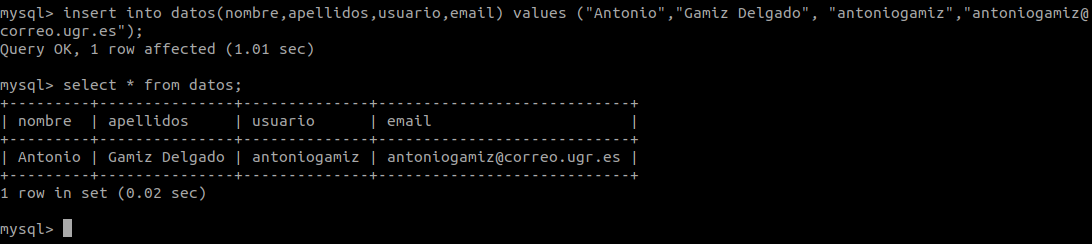
\includegraphics[scale=0.5]{img/3.png}
%\end{figure}

\end{document}
